\PassOptionsToPackage{dvipsnames}{xcolor}
\documentclass[aspectratio=169,10pt]{beamer}

\newcommand{\teamname}{Binary}
\newcommand{\topicchoice}{Topic 4 -- Async Research Assistant}
\newcommand{\memberone}{Orkhan Aliyev}
\newcommand{\membertwo}{Habil Huseynov}
\newcommand{\repolink}{github.com/mrorxan/research-assistant}

\newcommand{\coursecode}{AI-ENG-110}
\newcommand{\coursename}{Software Engineering}
\newcommand{\institution}{AI Academy, National AI Center}
\newcommand{\semester}{Spring 2026}

\usepackage[T1]{fontenc}
\usepackage[utf8]{inputenc}
\usepackage{lmodern}
\usepackage[scaled=0.94]{helvet}
\usepackage{xcolor}
\usepackage{tabularx}
\usepackage{booktabs}
\usepackage{listings}
\usepackage{tikz}
\usetikzlibrary{shapes.geometric,arrows.meta,positioning,fit,backgrounds}

\usetheme{default}
\setbeamertemplate{navigation symbols}{}

\definecolor{accent}{HTML}{0B3D91}
\definecolor{soft}{HTML}{F2F4F8}
\definecolor{ok}{HTML}{166534}
\definecolor{barmuted}{HTML}{9AA5B1}

\setbeamercolor{title}{fg=accent}
\setbeamercolor{frametitle}{fg=accent}
\setbeamercolor{itemize item}{fg=accent}
\setbeamercolor{itemize subitem}{fg=accent}
\setbeamercolor{enumerate item}{fg=accent}
\setbeamercolor{block title}{bg=accent,fg=white}
\setbeamercolor{block body}{bg=soft,fg=black}

\setbeamerfont{title}{size=\Large,series=\bfseries}
\setbeamerfont{frametitle}{size=\large,series=\bfseries}

\setbeamertemplate{footline}{%
  \hfill{\scriptsize\color{black!60}\insertframenumber\,/\,\inserttotalframenumber}\hspace*{3ex}\vskip4pt%
}

\definecolor{codegreen}{rgb}{0,0.55,0}
\definecolor{codepurple}{rgb}{0.55,0,0.78}
\lstdefinestyle{python}{
  language=Python,
  backgroundcolor=\color{soft},
  commentstyle=\color{codegreen},
  keywordstyle=\color{accent},
  stringstyle=\color{codepurple},
  basicstyle=\ttfamily\scriptsize,
  breaklines=true,
  showstringspaces=false,
  frame=single,
  framerule=0.4pt,
  rulecolor=\color{black!30},
}

\begin{document}

% Slide 1: title. Speaker: Orkhan.
\begin{frame}
  \begin{center}
    \vspace{0.4cm}
    {\small \textsc{\institution}}\\[0.2em]
    {\small \textsc{\coursecode{} -- \coursename{} -- \semester{}}}\\[1.1em]
    \rule{0.7\textwidth}{0.6pt}\\[0.4em]
    {\Huge\bfseries\color{accent} \topicchoice}\\[0.4em]
    \rule{0.7\textwidth}{0.6pt}\\[1.1em]
    {\large Team \teamname}\\[0.5em]
    {\normalsize \memberone\quad\textbullet\quad\membertwo}\\[0.9cm]
    {\footnotesize\itshape Final Project Defense -- July 2026}\\[0.3em]
    {\footnotesize\texttt{\repolink}}
  \end{center}
\end{frame}

% Slide 2: the problem. Speaker: Orkhan.
\begin{frame}{The problem in one sentence}
  \begin{block}{What the system does}
    Ask a research question; we fetch Wikipedia, arXiv, and a web search
    \textbf{in parallel}, then an LLM writes a short answer where
    \textbf{every claim carries a [N] citation} back to a real source.
  \end{block}

  \vspace{0.6em}
  \begin{columns}[T,onlytextwidth]
  \column{0.31\textwidth}
  \textbf{In}
  \begin{itemize}
    \item One question, $\le$ 500 chars
    \item Optional \texttt{--sources wiki,arxiv}
  \end{itemize}

  \column{0.33\textwidth}
  \textbf{Out}
  \begin{itemize}
    \item Cited answer + references
    \item Timing, cache state, failures
  \end{itemize}

  \column{0.30\textwidth}
  \textbf{Why}
  \begin{itemize}
    \item LLMs alone hallucinate
    \item Grounding in sources = RAG
  \end{itemize}
  \end{columns}

  \vspace{0.9em}
  \centering
  \texttt{python -m researcher ask "..."}\\[0.3em]
  {\footnotesize Gemini 2.5 Flash Lite + Tavily, swappable by env var}
\end{frame}

% Slide 3: architecture. Speaker: Orkhan.
\begin{frame}{Architecture: one job per layer}
  \begin{columns}[T,onlytextwidth]
  \column{0.63\textwidth}
  \begin{center}
  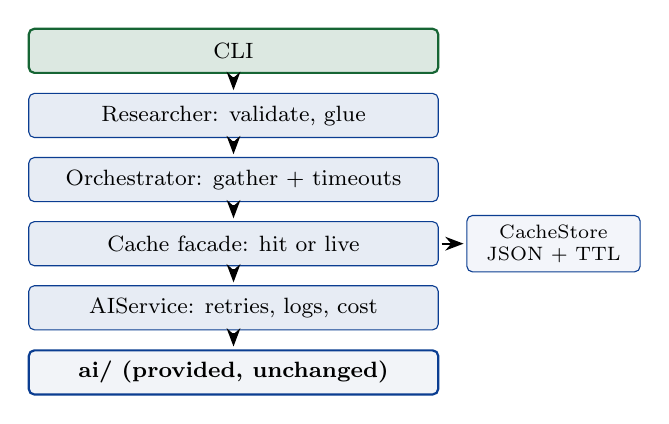
\begin{tikzpicture}[
    node distance=2.4mm,
    box/.style={draw,rounded corners=2pt,minimum width=5.2cm,minimum height=0.56cm,align=center,font=\footnotesize},
    aibox/.style={box,fill=soft,draw=accent,thick},
    sebox/.style={box,fill=accent!10,draw=accent},
    entry/.style={box,fill=ok!15,draw=ok,thick},
    side/.style={box,fill=accent!5,draw=accent,minimum width=2.2cm,font=\scriptsize},
    arrow/.style={-Stealth,thick,shorten <=1pt,shorten >=1pt}
  ]
    \node[entry] (cli) {CLI};
    \node[sebox,below=of cli] (core) {Researcher: validate, glue};
    \node[sebox,below=of core] (orch) {Orchestrator: gather + timeouts};
    \node[sebox,below=of orch] (cache) {Cache facade: hit or live};
    \node[sebox,below=of cache] (svc) {AIService: retries, logs, cost};
    \node[aibox,below=of svc] (ai) {\textbf{ai/ (provided, unchanged)}};
    \node[side,right=0.35cm of cache] (store) {CacheStore\\JSON + TTL};
    \draw[arrow] (cli) -- (core);
    \draw[arrow] (core) -- (orch);
    \draw[arrow] (orch) -- (cache);
    \draw[arrow] (cache) -- (svc);
    \draw[arrow] (svc) -- (ai);
    \draw[arrow] (cache) -- (store);
  \end{tikzpicture}
  \end{center}

  \column{0.34\textwidth}
  \vspace{0.3em}
  \textbf{Three hard boundaries}
  \begin{itemize}\setlength\itemsep{0.45em}
    \item Only \textbf{one module} imports \texttt{ai/}
    \item Only the facade touches storage
    \item Only the orchestrator spawns tasks
  \end{itemize}

  \vspace{0.7em}
  \begin{block}{Consequence}
    Swapping the LLM provider = one env var, zero code changes.
  \end{block}
  \end{columns}
\end{frame}

% Slide 4: design decisions. Speaker: Orkhan.
\begin{frame}{Three design decisions we can defend}
  \begin{enumerate}\setlength\itemsep{0.8em}
    \item \textbf{asyncio, not threads.}\\
      Three I/O-bound HTTP calls per question. One event loop, no GIL contention,
      and the provided fetchers are already coroutines.
    \item \textbf{A timeout per task, and one for the LLM too.}\\
      Each source gets its own \texttt{asyncio.timeout}, so a slow Wikipedia cannot
      cancel a fast arXiv. The synthesis call has its own 60\,s bound.
    \item \textbf{Filesystem JSON cache, and never cache empty results.}\\
      Entries are idempotent within their TTL, so no database needed. An empty
      result means a bad moment; remembering it for 24\,h would serve nothing
      after the source recovers.
  \end{enumerate}
\end{frame}

% Slide 5: wrapping ai/. Speaker: Orkhan (end of first half).
\begin{frame}{Wrapping the AI module: the service layer}
  \centering
  \begin{tabular}{ll}
    \toprule
    \textbf{Policy} & \textbf{Where it lives} \\
    \midrule
    Retries: 3 attempts, backoff 1--8\,s, only on \texttt{ProviderError} & AIService \\
    Programmer errors (\texttt{ValueError}) are \textbf{not} retried & AIService \\
    Cache by (source, canonicalised query), TTL 24\,h & Cache facade + store \\
    Cost record per LLM call, \texttt{cost-report} command & CostMeter \\
    Structured key=value logs, never a secret & everywhere \\
    \bottomrule
  \end{tabular}

  \vspace{1.0em}
  \begin{block}{Learned the hard way, live}
    Wikipedia returns \textbf{HTTP 403} unless the User-Agent identifies you with a
    contact. One shared \texttt{httpx} client now carries a policy-compliant agent
    for all three fetchers.
  \end{block}

  \vspace{0.4em}
  {\footnotesize Handover point: this layer tested, the second half composes it into an app.}
\end{frame}

% Slide 6: concurrency benchmark. Speaker: Habil (start of second half).
\begin{frame}{Concurrency: the benchmark}
  \textbf{Workload:} 5 asks $\times$ 3 stub sources, 0.5\,s sleep each.
  Deterministic, so it measures \emph{our orchestrator}, not the network.

  \vspace{0.9em}
  \begin{center}
  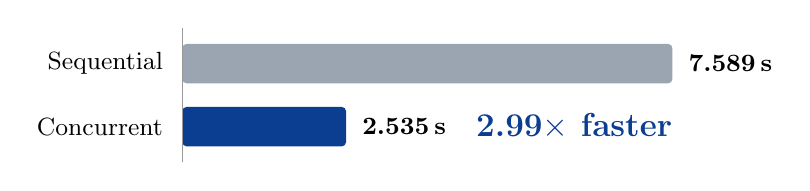
\begin{tikzpicture}[x=0.82cm]
    \draw[fill=barmuted,draw=none,rounded corners=1.5pt] (0,1.05) rectangle (7.589,1.55);
    \node[anchor=east,font=\small] at (-0.15,1.30) {Sequential};
    \node[anchor=west,font=\small\bfseries] at (7.689,1.30) {7.589\,s};
    \draw[fill=accent,draw=none,rounded corners=1.5pt] (0,0.25) rectangle (2.535,0.75);
    \node[anchor=east,font=\small] at (-0.15,0.50) {Concurrent};
    \node[anchor=west,font=\small\bfseries] at (2.635,0.50) {2.535\,s};
    \node[anchor=west,font=\large\bfseries,color=accent] at (4.4,0.50) {2.99$\times$ faster};
    \draw[black!40] (0,0.05) -- (0,1.75);
  \end{tikzpicture}
  \end{center}

  \vspace{0.7em}
  \begin{itemize}\setlength\itemsep{0.35em}
    \item Theoretical maximum with 3 equal sources is 3$\times$: \textbf{the fan-out costs nothing}.
    \item Live runs: 3.6--5.1\,s per question, about half of it the LLM call.
    \item New bottleneck: the slowest source + synthesis, not fetch parallelism.
  \end{itemize}

  \vspace{0.3em}
  {\footnotesize Reproduce without any API key: \texttt{python scripts/bench.py --N 5 --max-parallel 3}}
\end{frame}

% Slide 7: robustness. Speaker: Habil.
\begin{frame}[fragile]{Robustness: the failure found us}
  \textbf{Live incident, July 20.} Gemini returned 503 twice during a demo ask.

  \begin{lstlisting}[style=python,numbers=none,basicstyle=\ttfamily\scriptsize]
13:36:49 WARNING Retrying in 1 seconds ... 503 UNAVAILABLE
13:36:52 WARNING Retrying in 2 seconds ... 503 UNAVAILABLE
13:36:56 INFO    synthesize_done n_citations=2
  \end{lstlisting}

  The user saw a slower answer, not a crash.

  \vspace{0.6em}
  \textbf{The same discipline on every path}
  \begin{itemize}\setlength\itemsep{0.3em}
    \item One source fails or times out: the other two still answer, the output says so.
    \item All sources fail: clean error, exit code 3. Bad input: exit code 2.
    \item Windows console crashed on a Unicode arrow from the LLM: CLI now forces UTF-8.
    \item Bonus: \texttt{FailoverLLM} chains a second provider when configured; chaos-tested.
  \end{itemize}
\end{frame}

% Slide 8: sample run. Speaker: Habil.
\begin{frame}[fragile]{Sample run (real output)}
  \begin{lstlisting}[style=python,numbers=none,basicstyle=\ttfamily\scriptsize]
$ python -m researcher ask "What is photosynthesis and what are its main stages?"

A: Photosynthesis is a system of biological processes where
   photopigment-bearing organisms convert light energy into
   chemical energy [1]. [...] The main stages are the
   light-dependent reactions and the Calvin cycle [5, 6].

References:
  [1] (wikipedia) Photosynthesis -- en.wikipedia.org/wiki/Photosynthesis
  [5] (web) Photosynthesis -- education.nationalgeographic.org/...
  [6] (web) The process of photosynthesis -- monash.edu/...

timings: 9210 ms | cache: wikipedia=miss, arxiv=miss, web=miss
  \end{lstlisting}

  \vspace{0.4em}
  \begin{itemize}\setlength\itemsep{0.3em}
    \item Second identical ask: \texttt{arxiv=hit, web=hit}, 4.8\,s.
    \item All 5 sample questions answered live; records in \texttt{artefacts/demo\_run.json}.
    \item Estimated cost per question: about \$0.0002.
  \end{itemize}
\end{frame}

% Slide 9: testing. Speaker: Habil.
\begin{frame}{Testing and quality gates}
  \begin{columns}[T,onlytextwidth]
  \column{0.52\textwidth}
  \textbf{Numbers}
  \begin{itemize}\setlength\itemsep{0.35em}
    \item \textbf{92 tests}: 76 ours + 16 provided smoke
    \item Coverage on \texttt{researcher/}: \textbf{96\,\%}
    \item \texttt{mypy}: 0 issues \quad \texttt{ruff}: 0 findings
    \item All offline; \texttt{ai.*} boundary is mocked
    \item Same 92 pass \textbf{inside the Docker image}
  \end{itemize}

  \column{0.44\textwidth}
  \textbf{Tests worth naming}
  \begin{itemize}\setlength\itemsep{0.35em}
    \item Timeout isolates one source, others deliver
    \item \texttt{ValueError} is never retried
    \item Empty results are not cached
    \item Failover chaos test: primary dies, secondary answers
  \end{itemize}
  \end{columns}

  \vspace{0.8em}
  \begin{block}{CI on every pull request}
    ruff + mypy + pytest with a 60\,\% coverage gate + smoke tests + Docker build.
  \end{block}
\end{frame}

% Slide 10: limitations. Speaker: Habil.
\begin{frame}{Limitations \& what we would do next}
  \textbf{Honest weak spots}
  \begin{itemize}\setlength\itemsep{0.35em}
    \item Wikipedia title search often returns nothing for long questions; we degrade gracefully.
    \item No streaming: the user waits silently during synthesis.
    \item Cache has no cross-process lock (harmless at CLI scale, documented).
    \item Token counts are estimates; the fixed \texttt{ai/} interface hides real usage.
  \end{itemize}

  \vspace{0.7em}
  \textbf{Given another week}
  \begin{enumerate}\setlength\itemsep{0.35em}
    \item Query rewriting for Wikipedia recall.
    \item Streaming synthesis output to the terminal.
    \item Failover on by default with a second funded provider.
  \end{enumerate}
\end{frame}

% Slide 11: contributions. Speakers: both.
\begin{frame}{Team contributions: first half / second half}
  \begin{columns}[T,onlytextwidth]
  \column{0.48\textwidth}
  \textbf{Orkhan -- foundation \& service layer}
  \begin{itemize}\setlength\itemsep{0.3em}
    \item Project scaffold, config, models
    \item Cache store + cost telemetry
    \item AIService: retries, timeouts, logs
    \item Cache facade + their test files
    \item Report \S 1, 2, 4, 5; slides 1--5
  \end{itemize}

  \column{0.48\textwidth}
  \textbf{Habil -- composition \& shipping}
  \begin{itemize}\setlength\itemsep{0.3em}
    \item Orchestrator, Researcher flow, CLI
    \item FailoverLLM, demo + bench scripts
    \item Dockerfile, CI workflow, docs
    \item Their test files, live demo runs
    \item Report \S 3, 6, 7, 8; slides 6--10
  \end{itemize}
  \end{columns}

  \vspace{0.9em}
  \begin{block}{The handover}
    Orkhan built and tested everything up to the service layer; Habil composed it
    into the concurrent app and shipped it. Commits split accordingly, roughly 50/50.
  \end{block}
\end{frame}

% Slide 12: Q&A.
\begin{frame}
  \begin{center}
    \vspace{0.9cm}
    {\Huge\bfseries\color{accent} Questions?}\\[1.2em]
    \rule{0.5\textwidth}{0.6pt}\\[1.2em]
    {\large Team \teamname}\\[0.6em]
    {\normalsize \texttt{\repolink}}\\[0.8em]
    {\footnotesize\itshape Pick any file in the repo; we will walk through it.}
  \end{center}
\end{frame}

\end{document}